\documentclass{article}\usepackage[]{graphicx}\usepackage[]{color}
%% maxwidth is the original width if it is less than linewidth
%% otherwise use linewidth (to make sure the graphics do not exceed the margin)
\makeatletter
\def\maxwidth{ %
  \ifdim\Gin@nat@width>\linewidth
    \linewidth
  \else
    \Gin@nat@width
  \fi
}
\makeatother

\definecolor{fgcolor}{rgb}{0.345, 0.345, 0.345}
\newcommand{\hlnum}[1]{\textcolor[rgb]{0.686,0.059,0.569}{#1}}%
\newcommand{\hlstr}[1]{\textcolor[rgb]{0.192,0.494,0.8}{#1}}%
\newcommand{\hlcom}[1]{\textcolor[rgb]{0.678,0.584,0.686}{\textit{#1}}}%
\newcommand{\hlopt}[1]{\textcolor[rgb]{0,0,0}{#1}}%
\newcommand{\hlstd}[1]{\textcolor[rgb]{0.345,0.345,0.345}{#1}}%
\newcommand{\hlkwa}[1]{\textcolor[rgb]{0.161,0.373,0.58}{\textbf{#1}}}%
\newcommand{\hlkwb}[1]{\textcolor[rgb]{0.69,0.353,0.396}{#1}}%
\newcommand{\hlkwc}[1]{\textcolor[rgb]{0.333,0.667,0.333}{#1}}%
\newcommand{\hlkwd}[1]{\textcolor[rgb]{0.737,0.353,0.396}{\textbf{#1}}}%

\usepackage{framed}
\makeatletter
\newenvironment{kframe}{%
 \def\at@end@of@kframe{}%
 \ifinner\ifhmode%
  \def\at@end@of@kframe{\end{minipage}}%
  \begin{minipage}{\columnwidth}%
 \fi\fi%
 \def\FrameCommand##1{\hskip\@totalleftmargin \hskip-\fboxsep
 \colorbox{shadecolor}{##1}\hskip-\fboxsep
     % There is no \\@totalrightmargin, so:
     \hskip-\linewidth \hskip-\@totalleftmargin \hskip\columnwidth}%
 \MakeFramed {\advance\hsize-\width
   \@totalleftmargin\z@ \linewidth\hsize
   \@setminipage}}%
 {\par\unskip\endMakeFramed%
 \at@end@of@kframe}
\makeatother

\definecolor{shadecolor}{rgb}{.97, .97, .97}
\definecolor{messagecolor}{rgb}{0, 0, 0}
\definecolor{warningcolor}{rgb}{1, 0, 1}
\definecolor{errorcolor}{rgb}{1, 0, 0}
\newenvironment{knitrout}{}{} % an empty environment to be redefined in TeX

\usepackage{alltt}
\usepackage[margin=1in]{geometry}
\usepackage{graphicx, hyperref, float, multicol, pdflscape, paralist}
\usepackage[backend=bibtex, natbib=true]{biblatex}
\addbibresource{references/refs.bib}

\usepackage{color}
\newcommand{\hh}[1]{{\color{magenta} #1}}
\newcommand{\ak}[1]{{\color{blue} #1}}

\title{gravicom - a web-based tool for community detection in networks}
\author{Andrea J. Kaplan}
\IfFileExists{upquote.sty}{\usepackage{upquote}}{}

\begin{document}

\maketitle
\section{Background}
\subsection{Networks}
\subsection{Visualization}
\subsection{Layout Algorithms}

\section{User Interface}
\subsection{Design and Functionality}

Before discussing gravicom's performance and use on example datasets, we give a brief overview of the components and functionality that make up the tool.



\subsubsection{Description}

The gravicom interface is comprised of five main parts,
\begin{enumerate}
\item Control panel
\item Data management
\item Connection table 
\item Graph display
\item Tabset.
\end{enumerate}

\begin{figure}[H]
\centering
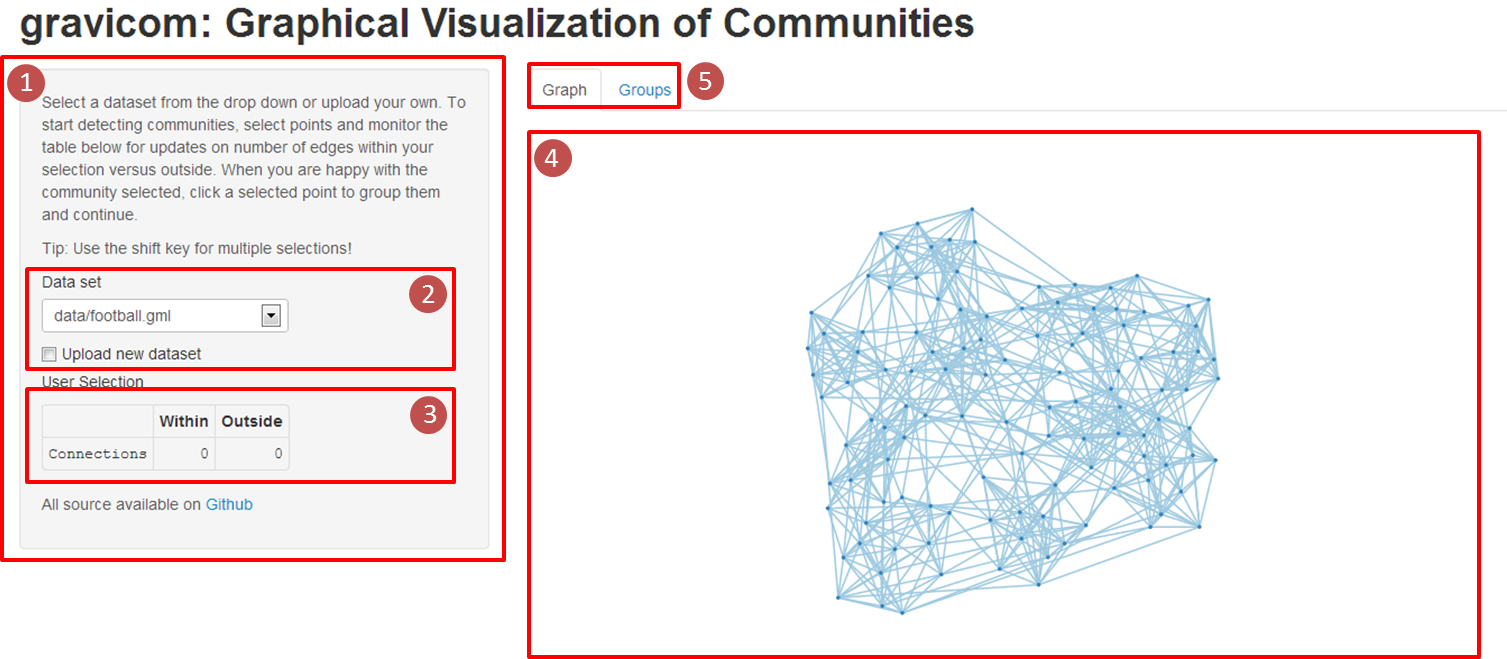
\includegraphics[width=\textwidth]{images/sitecomponents.png}
\caption{\label{fig:sitecomponents} The components that make up gravicom, (1) Control panel, (2) Data management, (3) Connection table, (4) Graph display, and (5) Tabset.}
\end{figure}

Each part provides a means for the user to interact with gravicom, either through controls that allow user input to gravicom or through direct interaction with diagnostics and visualization of a graph. Their placement on the gravicom interface can be seen in Figure~\ref{fig:sitecomponents}.

\paragraph{Control Panel}
The control panel serves as the starting point for a user's session in gravicom. It contains intructions for the user, as well as the means for a user to select a dataset and numerical summaries of the graph (such as a diagnostic connection table explained below). Additionally, the control panel contains a link to the source code for gravicom, should a user be interested in the inner workings of gravicom.

\paragraph{Data Management}
The data management component is made up of two main parts, data selection and data download. The data selection can be accomplished in two ways, the first being a drop down to select pre-loaded datasets to display. Currently there are two well-known network datasets provided in gravicom, a college football dataset \cite{gn-football} and a karate club dataset \cite{zachary1977information}. From the dropdown the user can change the dataset to display in the graph. The second approach to data selection gives the user the ability to upload his own dataset. Upon clicking the ``Upload new dataset" checkbox, a file selection control appears which gives the user the ability to upload his own graph data to explore with gravicom. This is shown in Figure~\ref{fig:uploadnewdataset}. 

\begin{figure}[H]
\centering

\includegraphics[]{images/uploadnewdataset.png}
\caption{\label{fig:uploadnewdataset} The data selection area upon clicking the ``Upload new dataset" checkbox.}
\end{figure}

The work performed by a user in visualizing graphs and community structure can also be downloaded as a dataset from gravicom with current communities stored. This feature can be used as a save point in processing a graph or as a means to export changes made in gravicom to another tool.

\paragraph{Connection Table}
The connection table is a quantitative diagnostic tool for the user in assessing the strength of a community structure in a graph. The idea behind the connection table is that a community of nodes will have proportionally more edge connections within the node cluster compared to edge connections to nodes outside the community. The table displays the number of edge connections within a user's selection of nodes in the graph and the number of connections from nodes in a user's selection to nodes not in the selection. The comparison of these two numbers can give the user a rough idea of if the plausibiity or extend to which the node selection constitutes a community. To aid in the comparison, there is also a proportion column that displays the ratio of number of connections within a node selection to the number of connections outside the selection. 

\paragraph{Graph Display} \label{par:graph}
The graph display shows an interactive graphical representation of  the selected (or uploaded) graph data. Upon load, the graph displays all nodes and edges in the dataset using a force-directed layout algorithm. The user has several ways to interact with the graph: drag, select, and group. A user can drag a node at any time. Upon dragging, the force-directed layout is  rerun, giving an altered view of the graph. Figure~\ref{fig:graphdrag} shows a graph in the process of being dragged.

\begin{figure}[H]
\centering
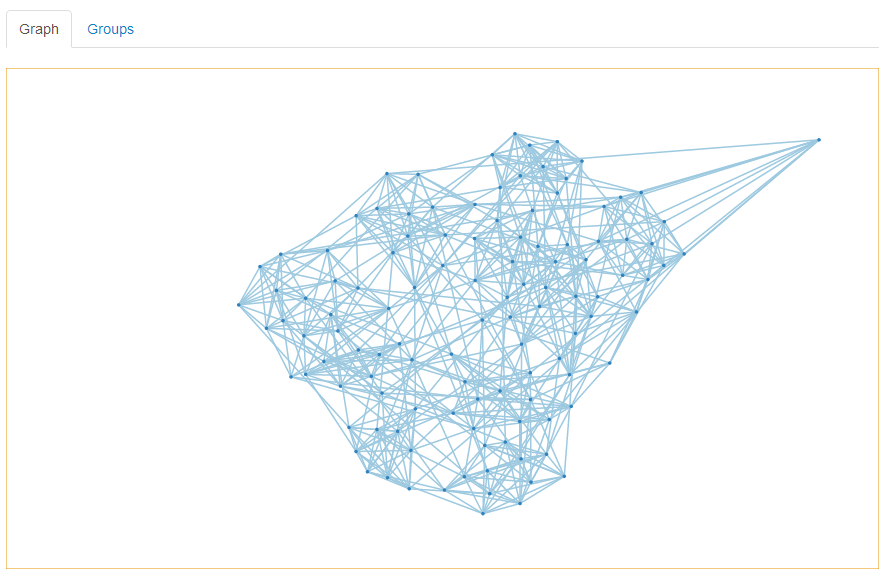
\includegraphics[width=\textwidth]{images/graphdrag.png}
\caption{\label{fig:graphdrag} A graph in the process of being dragged. The node being dragged is marked by a red circle.}
\end{figure}

Selection and grouping of nodes are actions intended to work todether. In order to group nodes, a user first determines a node cluster or potential community based on a visual appraisal of the graph. To select nodes the user clicks and drags a selection box around nodes. See Figure~\ref{fig:graphselect} for the results of selection in the interface. The shift key can also be used for multiple selections. Upon selection, the connection table is updated and the user can evaluate the selection as a community and alter the selection if need be (the shift key selection is useful in this step).

\begin{figure}[H]
\centering
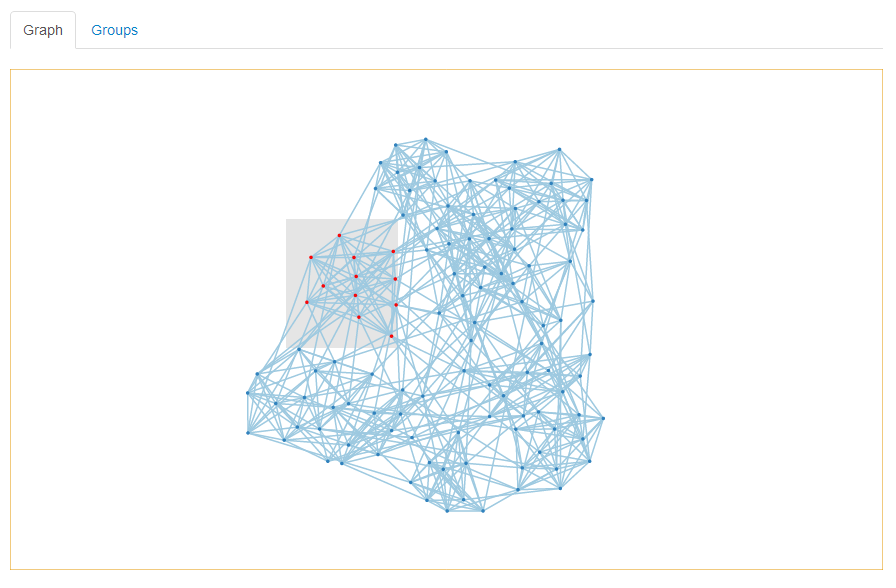
\includegraphics[width=\textwidth]{images/graphselect.png}
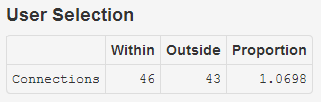
\includegraphics[]{images/tableselect.png}
\caption{\label{fig:graphselect} A graph in the process of nodes being selected. Upon selection of nodes, the connection table updates to display within and outside edges.}
\end{figure}

Selected nodes can be grouped together into one consolidated ``super-node" or grouped-node. Once grouped, the size and edges of the super-node represent the number of nodes in the potential community and the number of edges to the grouped community nodes, respectively. The force-directed layout is again run, showing the new graph with previous nodes grouped. This is illustrated in Figure~\ref{fig:graphgroup}. This process of node grouping can be repeated until all nodes have been grouped or until the user is satisfied that all communities have been selected. Additionally, grouped nodes can be ungrouped by clicking on a grouped node. 

\begin{figure}[H]
\centering
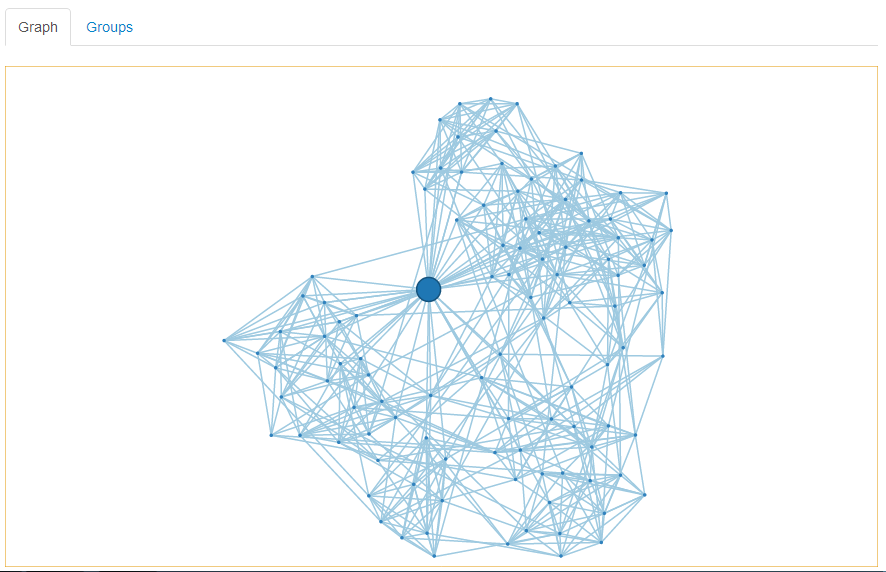
\includegraphics[width=\textwidth]{images/graphgroup.png}
\caption{\label{fig:graphgroup} A graph after nodes have been grouped and the force-directed algorithm has been re-run.}
\end{figure}

\paragraph{Tabset} \label{par:group}
The tabset allows the user to switch between two tabs on the screen. The first (and default tab) shows the graph display. The second tab shows the groups that a user has created in the graph. Within this tab, each node group or community summarizes the number of nodes in the group and also provides the ability to drop down and view the node IDs for that group. If the data are equipped with node labels, these will be displayed. If there are no node labels provided, node IDs will be shown as node numbers. For an example, see Figure~\ref{fig:groupstab}.

\begin{figure}[H]
\centering
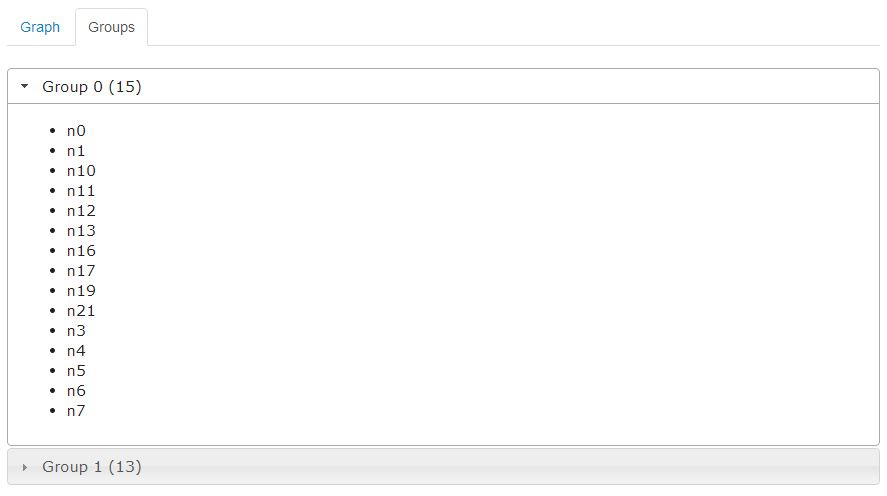
\includegraphics[width=\textwidth]{images/groupstab.png}
\caption{\label{fig:groupstab} The groups tabset displaying which nodes have been grouped in Group 0, for example. The groups tabset also shows that Group 0 has 15 nodes, while Group 1 has 13 nodes.}
\end{figure}


\section{Examples}

To demonstrate the use of gravicom, we present three real-world network datasets and explore their community structure.

\subsection{College Football} \label{sec:football}
The first dataset is a representation of U.S. College Football Division 1 games from the 2000 season \cite{gn-football}. This is a default dataset available in gravicom. In this network, nodes represent teams and an edge represents a regular-season game played between the two connected teams. The distances between the nodes are based on the number of games played between the teams. The network as it appears upon load in gravicom is presented in Figure~\ref{fig:football_1}. 

\begin{figure}[H]
\centering
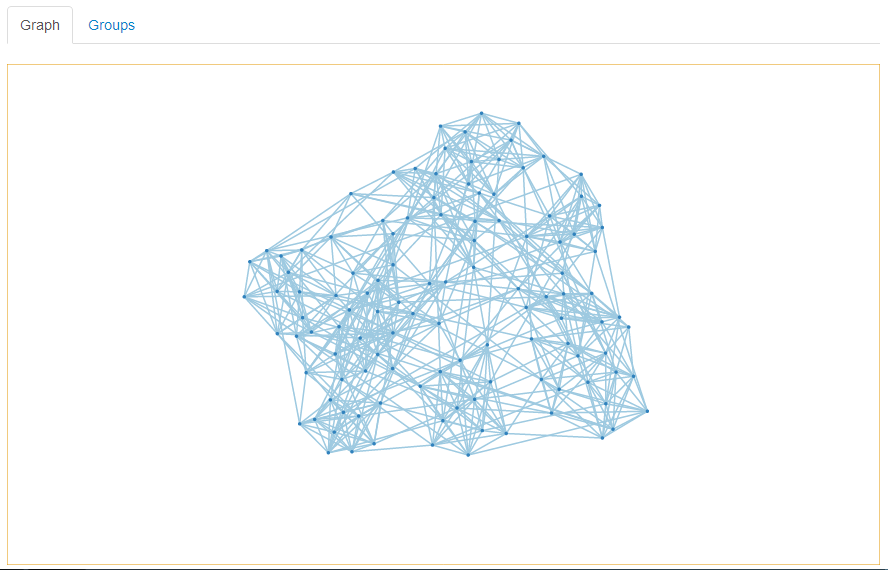
\includegraphics[width=0.6\textwidth]{images/football_1.png}
\caption{\label{fig:football_1} College Football network represented in gravicom. Communities are visually evident and will become more identifiable as other are grouped.}
\end{figure}

Colleges within the same football conference will play members of their conference more frequently than teams outside of their conference, making this an interesting dataset for attempting to visually detect community structures. This is also an ideal illustrative example due to the relatively small number of nodes and edges present, making a graphical representation particularly feasible. One challenge with this dataset, however is the existence of independent teams, like Notre Dame, which do not belong to any conference and so may complicate efforts of community detection. Another complication is that small conference schools typically play large conference schools at the beginning of a season in order to help fund their athletic programs, which can potentially cause more edges than perhaps expected between distinct communities, particularly between small conferences and large conferences.

Upon viewing the network in gravicom, some likely communities visually emerge, and by selecting nodes to examine within and outside edges, we can classify colleges into conferences, as seen in Figure~\ref{fig:football_2}.

\begin{figure}[H]
\centering
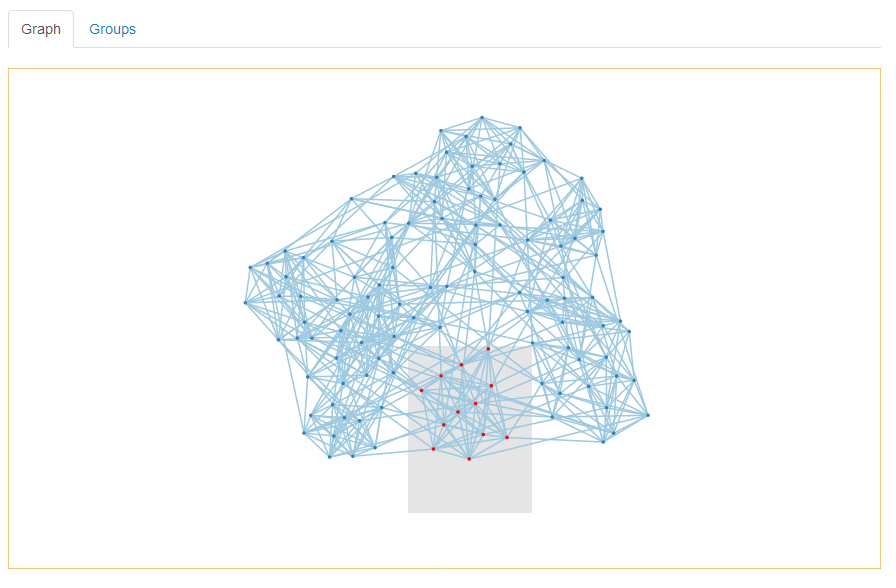
\includegraphics[width=.49\textwidth]{images/football_2.png}
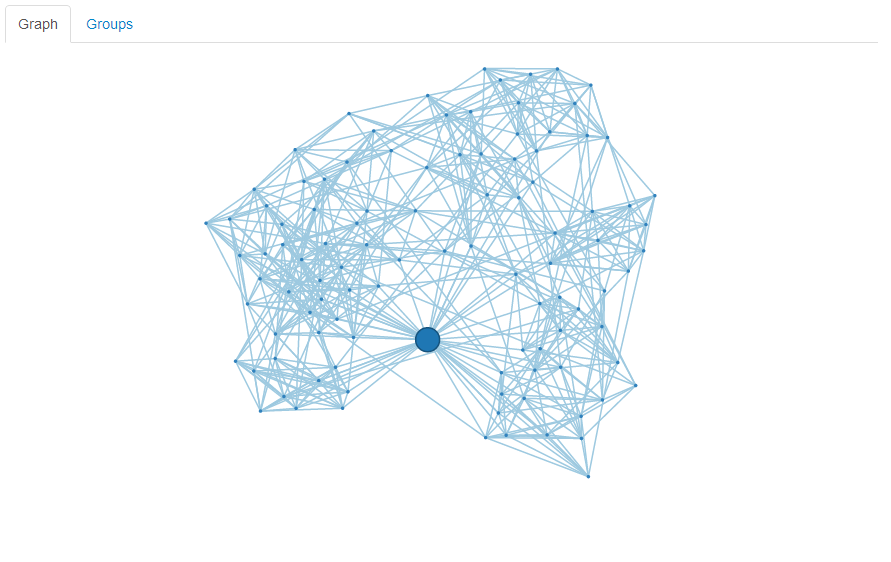
\includegraphics[width=.49\textwidth]{images/football_4.png}
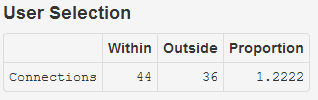
\includegraphics[]{images/football_3.png}
\caption{\label{fig:football_2} Selecting a potential community in gravicom and assessing the number of within verses outside selection edges. After the first community is detected, more communities become apparent in the network.}
\end{figure}

Once the user is satisfied that he has selected a viable community, he clicks to group those nodes and the graph will update to reflect this. In particular, the grouped nodes for the suspected community will be collapsed into one super-node in the updated graph. See Section~\ref{par:graph} for details. The resulting graph update allows new community structures to potentially become more easily apparent as seen in Figure~\ref{fig:football_2}. 

Additionally, the user can check which nodes were grouped in each community as described in \ref{par:group}. In this example, the first community detected contains the following schools, which corresponds to the Big 10:\begin{inparaenum}[\itshape a\upshape)]
\item Illinois;
\item Indiana; 
\item Iowa; 
\item Michigan; 
\item Michigan State; 
\item Minnesota; 
\item Northwestern; 
\item Ohio State; 
\item Penn State;
\item Purdue; and
\item Wisconsin.
\end{inparaenum}

After the first community has been selected, another potential community at the top of the graph has been revealed \ak{(explain)}. The user can once again select and group this node cluster into a community and subsequently examine the nodes in the resulting group as seen in Figure~\ref{fig:football_6}. The second conference grouped corresponds exactly to the SEC Conference, another large college football conference. Here, the first two communities to become evident correspond to large Division 1 conferences that play the majority of their games within conference, matching our earlier assertion that small conferences should, as expected, be more difficult to detect.

\begin{figure}[H]
\centering
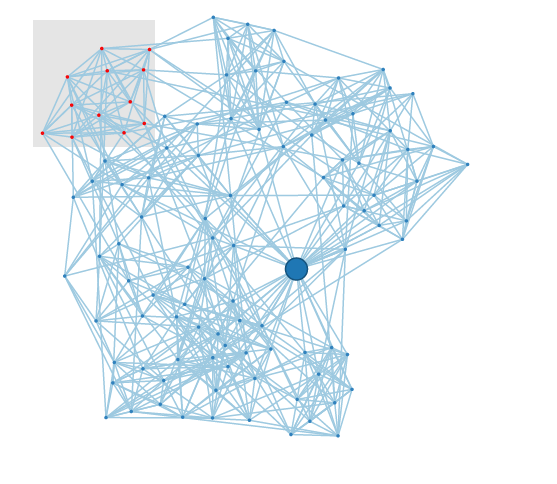
\includegraphics[width=.49\textwidth]{images/football_45.png}
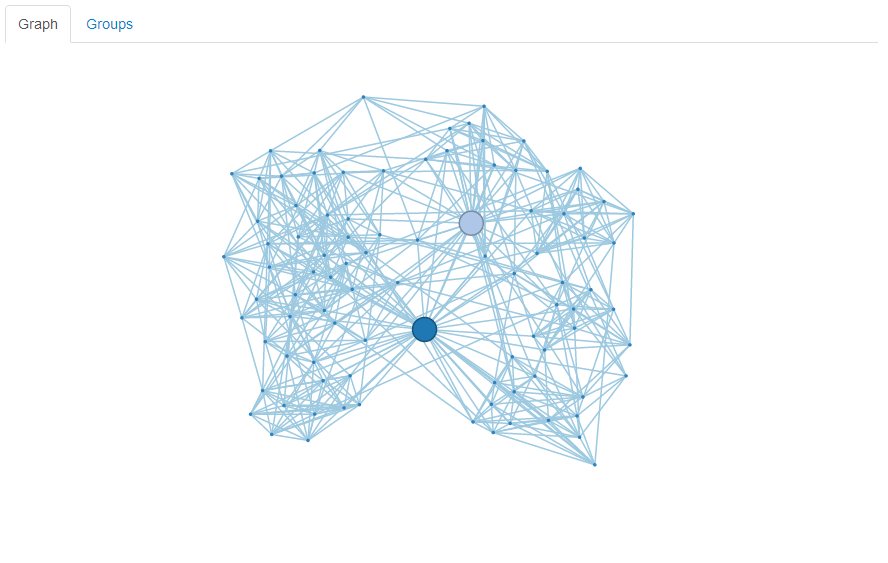
\includegraphics[width=.49\textwidth]{images/football_6.png}
\caption{\label{fig:football_6} A second community is grouped which corresponds to the SEC Conference.}
\end{figure}

This process of grouping nodes into suspected communities can be repeated until the user is satisfied with the communities selected. The entirety of this process is seen in Figure~\ref{fig:football_progression} and the resulting communities in Table~\ref{tab:football_final}. It should be noted that this is a fundamentally a subjective process and that another user with the same data may find slightly different communities. However, by leveraging the human visual system to find structure in a dataset, gravicom has the ability to provide a starting point for an objective algorithm to then adopt the detection of communities. 

\begin{figure}[H]
\centering
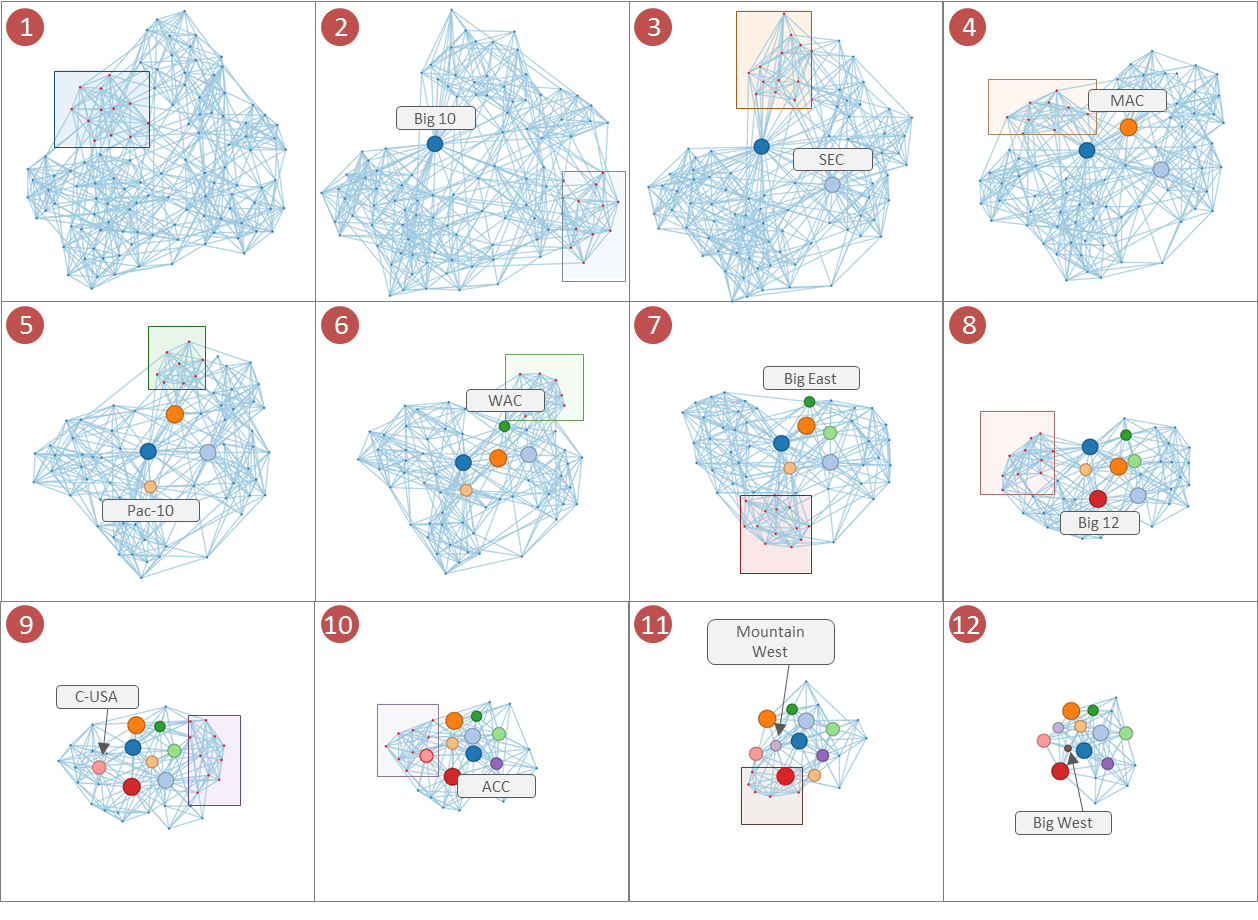
\includegraphics[width=\textwidth]{images/football_progression.png}
\caption{\label{fig:football_progression}The full process of selecting and grouping communities in gravicom using the football dataset.}
\end{figure}

% latex table generated in R 3.0.2 by xtable 1.7-1 package
% Sun Feb 09 17:10:13 2014
\begin{table}[H]
\centering
\begin{tabular}{cp{10cm}c}
  \hline
Conference & Teams Identified & Accuracy \\ 
  \hline
ACC & Duke,  Wake Forest,  Virginia,  Florida State,  Clemson,  North Carolina,  Maryland,  Georgia Tech,  North Carolina State & 100\% \\ 
  Big East & Boston College,  Miami Florida,  Virginia Tech,  Syracuse,  Temple,  West Virginia, {\it  Connecticut},  Pittsburgh,  Rutgers & 88.9\% \\ 
  Big 10 & Ohio State,  Penn State,  Michigan,  Michigan State,  Purdue,  Minnesota,  Northwestern,  Illinois,  Iowa,  Wisconsin,  Indiana & 100\% \\ 
  Big 12 & Kansas State,  Iowa State,  Kansas,  Texas A\& M,  Texas Tech,  Baylor,  Missouri,  Texas,  Oklahoma State,  Colorado,  Oklahoma,  Nebraska & 100\% \\ 
  C-USA & Cincinnati,  Louisville,  Houston,  Tulane,  Southern Mississippi,  Army,  Memphis,  East Carolina,  Alabama Birmingham & 100\% \\ 
  Independent & Notre Dame,  Navy & 100\% \\ 
  MAC & {\it  Central Florida},  Western Michigan,  Miami Ohio,  Ohio,  Bowling Green State,  Marshall,  Ball State,  Akron,  Buffalo,  Northern Illinois,  Eastern Michigan,  Toledo,  Central Michigan,  Kent & 92.9\% \\ 
  Mountain West & Brigham Young,  San Diego State, {\it  Boise State},  Wyoming,  New Mexico,  Nevada Las Vegas,  Utah, {\it  North Texas}, {\it  Utah State}, {\it  New Mexico State},  Colorado State, {\it  Arkansas State}, {\it  Idaho},  Air Force & 57.1\% \\ 
  Pac-10 & Arizona,  Oregon State,  Washington,  Washington State,  Arizona State,  UC LA,  Stanford,  Southern California,  Oregon,  California & 100\% \\ 
  SEC & Vanderbilt,  Florida,  Louisiana State,  South Carolina,  Mississippi,  Arkansas,  Auburn,  Kentucky,  Georgia,  Mississippi State,  Alabama,  Tennessee & 100\% \\ 
  Big West & Middle Tennessee State,  Louisiana Lafayette,  Louisiana Monroe, {\it  Louisiana Tech} & 75\% \\ 
  WAC & Nevada,  Fresno State, {\it  Texas Christian},  Tulsa,  Hawaii,  Rice,  Southern Methodist,  San Jose State,  Texas El Paso & 88.9\% \\ 
   \hline
\end{tabular}
\caption{Resulting communities detected using gravicom and the corresponding conference. Teams that have been incorrectly classified are italicized.} 
\label{tab:football_final}
\end{table}



Using the visual approach detailed above, we were able to detect 11 community structures in the graph. There were 11 conferences and 5 independent schools in the dataset. Through manual specification of conferences, we were able to correctly classify 91.3\% of the football teams into their conferences. 

\subsection{Political Books Sold}
For illustration, we next consider a second example dataset consisting of a network of political books purchased close to the 2004 United States presidential election and sold on Amazon.com \cite{polbooks}. Each node represents a book and each edge represents frequent copurchasing of two books by the same buyers. The books are classified as being conservative, liberal, or neutral by the author of the dataset \cite{krebs2004divided} and we can see a clear partition in Figure~\ref{fig:polbooks_1} between two main groups (i.e. roughly conservative and liberal) with a smaller group between, when looking at the network in gravicom. This dataset is interesting because it highlights a great divide in the United States population that can be ascribed to the two party political system. 

\begin{figure}[H]
\centering
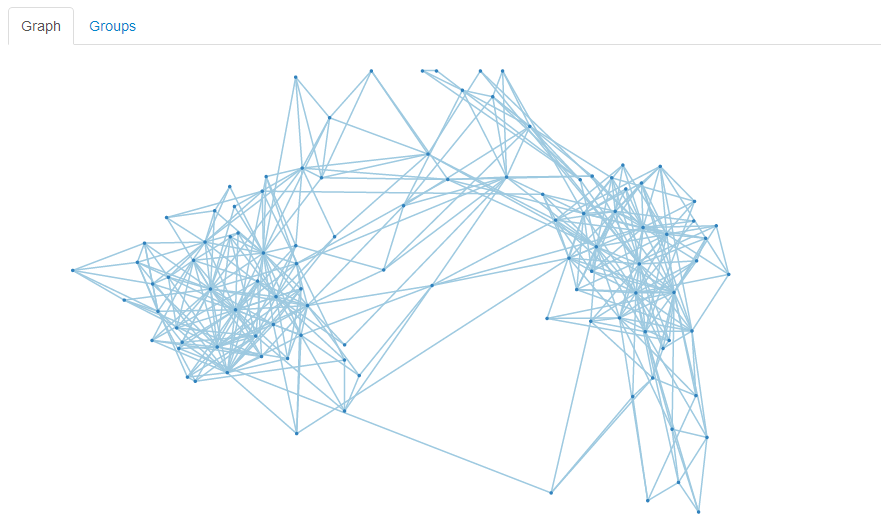
\includegraphics[width=\textwidth]{images/polbooks_1.png}
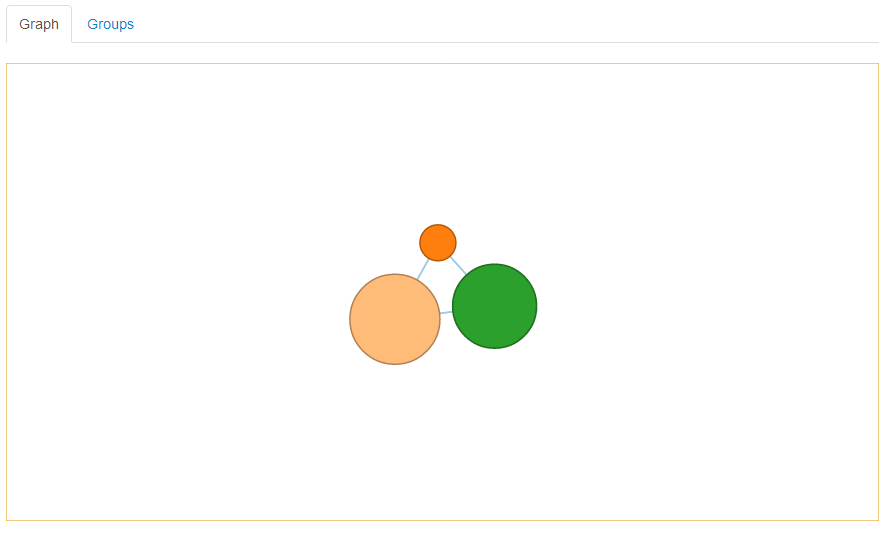
\includegraphics[width=\textwidth]{images/polbooks_2.png}
\caption{\label{fig:polbooks_1} Political books dataset as seen in gravicom prior and post community detection.}
\end{figure}

% latex table generated in R 3.0.2 by xtable 1.7-1 package
% Sun Feb 09 17:10:13 2014
\begin{table}[H]
\centering
\begin{tabular}{cp{10cm}c}
  \hline
Classification & Books Identified & Accuracy \\ 
  \hline
Conservative & A National Party No More, Dereliction of Duty, Ten Minutes from Normal, Bush Country, Rumsfeld's War, Legacy, Hating America, Hillary's Scheme, {\it Meant To Be}, Tales from the Left Coast, Breakdown, Losing Bin Laden, The French Betrayal of America, Spin Sisters, The Right Man, Useful Idiots, Shut Up and Sing, Who's Looking Out for You?, Those Who Trespass, Bias, The O'Reilly Factor, Let Freedom Ring, Deliver Us from Evil, Give Me a Break, Betrayal, The Real America, The Faith of George W Bush, The Death of Right and Wrong, {\it Power Plays}, Arrogance, {\it The Perfect Wife}, The Bushes, Things Worth Fighting For, Off with Their Heads, Persecution, Why Courage Matters, Hollywood Interrupted, The Enemy Within, We Will Prevail, Endgame, The Official Handbook Vast Right Wing Conspiracy, The Third Terrorist, Slander, The Savage Nation, Fighting Back & 93.3\% \\ 
  Liberal & Downsize This!, The Culture of Fear, House of Bush, House of Saud, The Best Democracy Money Can Buy, Rogue Nation, Stupid White Men, Rush Limbaugh Is a Big Fat Idiot, The Great Unraveling, Against All Enemies, American Dynasty, The Price of Loyalty, The Sorrows of Empire, Worse Than Watergate, {\it Plan of Attack}, Big Lies, The Lies of George W. Bush, Bushwomen, The Bubble of American Supremacy, Living History, The Politics of Truth, Fanatics and Fools, Bushwhacked, Disarming Iraq, Lies and the Lying Liars Who Tell Them, MoveOn's 50 Ways to Love Your Country, The Buying of the President 2004, Perfectly Legal, {\it Bush at War}, The New Pearl Harbor, Freethinkers, Had Enough?, It's Still the Economy, Stupid!, We're Right They're Wrong, What Liberal Media?, The Clinton Wars, Weapons of Mass Deception, Dude, Where's My Country?, Thieves in High Places, Shrub, Buck Up Suck Up, Hegemony or Survival, The Exception to the Rulers & 95.2\% \\ 
  Neutral & 1000 Years for Revenge, {\it Bush vs. the Beltway}, {\it Charlie Wilson's War}, {\it Dangerous Dimplomacy}, Sleeping With the Devil, {\it The Man Who Warned America}, Why America Slept, Ghost Wars, Surprise, Security, the American Experience, {\it Allies}, {\it The Choice}, All the Shah's Men, {\it Soft Power}, Colossus, The Future of Freedom, {\it Rise of the Vulcans}, {\it America Unbound}, Empire & 50\% \\ 
   \hline
\end{tabular}
\caption{Resulting communities detected using gravicom and the corresponding type of book. Books that have been incorrectly classified are italicized.} 
\label{tab:polbooks_final}
\end{table}


We detected visually 3 types of books in the dataset using the process of selection and grouping detailed in section~\ref{sec:football}. Through subsequent manual verification of the classification of books, we found that we were able to correctly classify 86.67\% of the books into the categories created by the author of the dataset. See Table~\ref{tab:polbooks_final} for the final groups of books found using gravicom.


\section{Technical Aspects}

gravicom utilizes three main pieces of software to establish interactive user control of a random graph as sketched out in Figure~\ref{fig:clientserver}, which are Shiny, D3, and igraph. These are used, respectively, for server/client interaction management, user interface and graph layout, and data formatting, respectively. In the following subsections, we describe the purposes of these three components in more detail.

\begin{figure}[H]
\centering
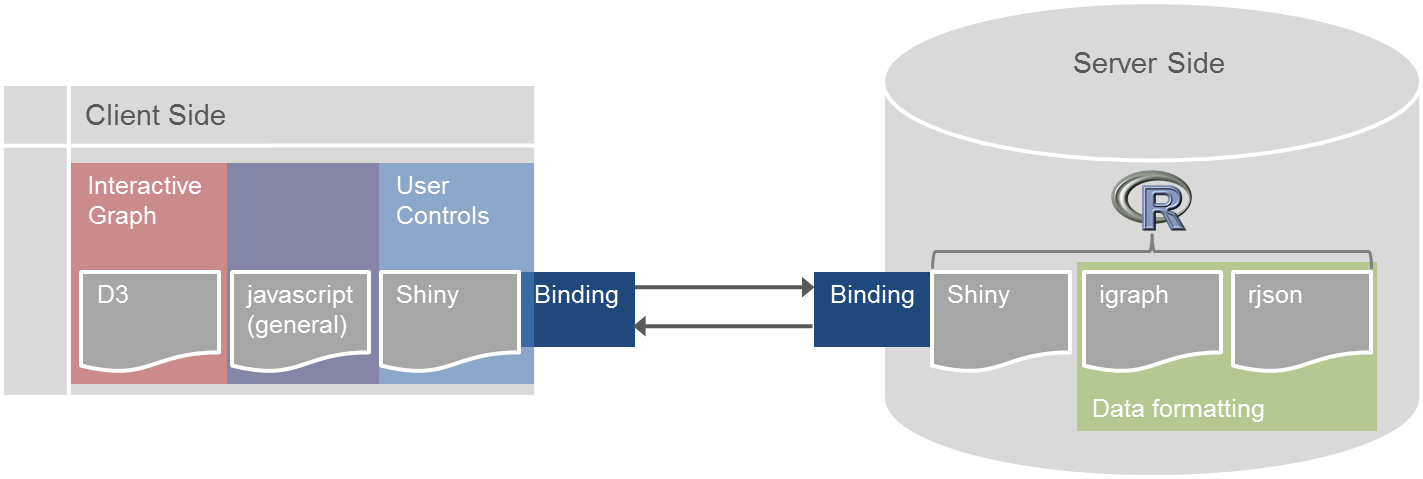
\includegraphics[width=\textwidth]{images/clientserverflow.png}
\caption{\label{fig:clientserver} Relationship between client and server, specifically focusing on how data travels between the two.}
\end{figure}

There are very minimal software requirements for a user of gravicom. The client simply needs to have a JavaScript enabled internet browser with HTML5 compatibility, something which almost any modern browser fulfills (an exception is IE8 and below). 

The server side requirements are more extensive, but this does not affect the user of gravicom, only those wanting to host their own instance of the application. To host gravicom, a Linux server is required, with the following installed:

\begin{itemize}
\item Node.js (0.8.16 or later)
\item {\tt R} (2.15 or later)
\item Shiny {\tt R} package, installed into the machine-wide site library. 
\item Shiny Server
\end{itemize}


\subsection{Shiny}

Shiny \cite{rs-shiny} is an {\tt R} package created by RStudio that enables {\tt R} users to create an interactive web application that utilizes {\tt R} as the background engine. Through default methods to build user interface elements in HTML and a handle to the server side code, Shiny is a simple way to turn {\tt R} code into a website. 

gravicom uses the Shiny functionality to create user controls, pass correctly formatted data to the client, and as a means to display summary information regarding the user's interactions with a graph at any point in time. In this context, Shiny serves as the translator between the formatted data and what the user sees and interacts with on his screen.


\subsection{D3}

D3 \cite{mb-d3} stands for ``Data Driven Documents" and is a JavaScript library developed and maintained by Mike Bostock with the  purpose of visualizing and interacting with data in a web-based interface. It is freely available from \url{http://www.d3js.org}. The library facilitates manipulation of HTML elements, SVG (scalable vector graphics), and CSS (cascading style sheets) with the end goal of rendering animations and providing user interactions that are tied to the underlying data. The key idea behind the library is that Document Object Model elements are completely determined by the data. The Document Object Model (DOM) is a convention for representing and interacting with objects in HTML, XHTML and XML. So, rather than adding elements to a web page to be viewed by users, D3 allows users to see and interact with graphical representations of their data in a web framework. 

gravicom uses D3 to handle all graphical displays and user interactions with the graph. The data is passed to the client and able to be used through Shiny's input bindings. It is crucial that the data has been formatted correctly at this point for the JavaScript to properly function. For this reason, we limit the file types being passed into the tool to a robust graph-specific type.

At this point in the page lifecycle, the graph nodes are tied to circles and the edges are tied to paths on the page. User manipulations such as selecting, dragging, and grouping are handled by D3 and  data is passed back to the server via Shiny's output bindings to allow for communication between user and the {\tt R} engine underneath. This is illustrated in Figure~\ref{fig:pagelifecycle}. What this means is that all visualization and user interaction with the graph are accomplished using JavaScript, more specifically the library D3. Shiny and {\tt R} serve as the framework on which the data sits, but when the user touches the data they are doing so through the JavaScript elements. 

\begin{figure}[H]
\centering
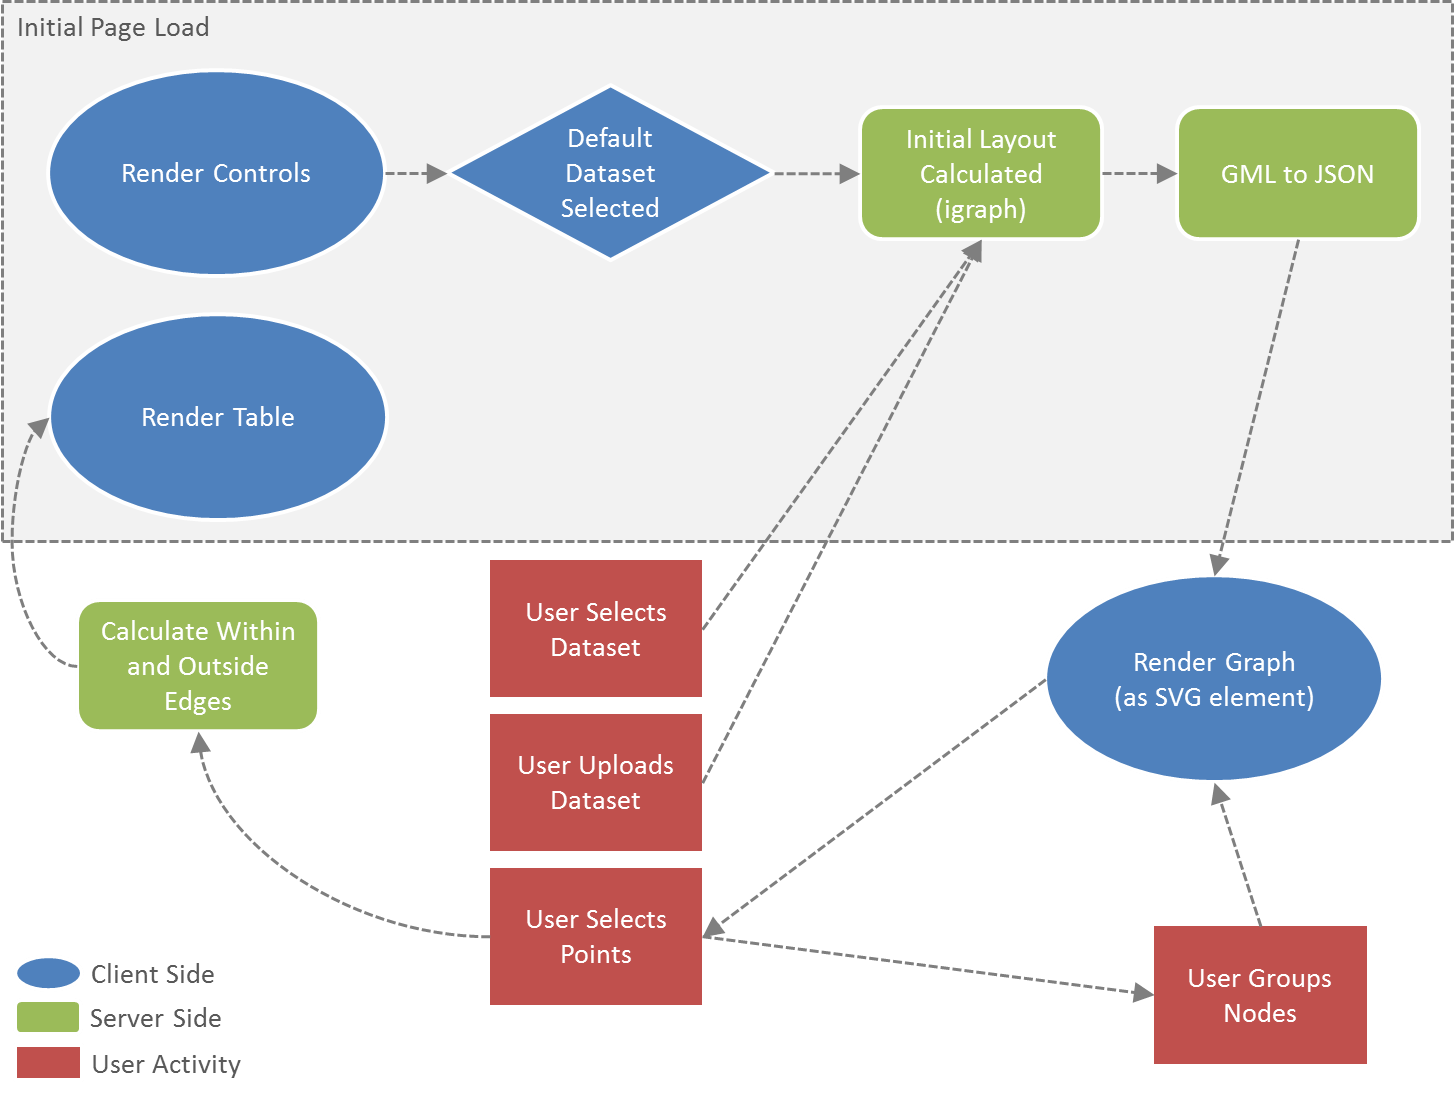
\includegraphics[width=\textwidth]{images/pagelifecycle.png}
\caption{\label{fig:pagelifecycle} Page lifecycle beginning from on load. User actions are highlighted in red, server actions in green, and actions completed on the client side are highlighted in blue.}
\end{figure}


\subsection{igraph}

igraph \cite{gc-igraph} is a software package used for creating and manipulating undirected and directed graphs. It is a cross-language package available for C, R, python, and Ruby. igraph also supports multiple graph file formats and visualization of graph structures.

gravicom utilizes two parts of igraph, first is the conversion from a gml file to an XML file. The gml file format, short for Graph Modelling Language, is a hierarchical ASCII-based file format for describing graphs. Below is an example gml file of an undirected graph consisting of two nodes linked by a single edge. The important points to note are that  node identifiers (id) have to be numeric. An edge consists only of source and target ids of the nodes it connects, while  nodes can have other attributes, e.g.~{\tt value} in the example. For a directed graph, the parameter {\tt directed} has to be set to 1, which will result in the edge information on target and source being evaluated accordingly.
\begin{knitrout}
\definecolor{shadecolor}{rgb}{0.969, 0.969, 0.969}\color{fgcolor}\begin{kframe}
\begin{verbatim}
## graph
## [
##   directed 0
##   node
##   [
##     id 0
##     label "Node 1"
##     value 100
##   ]
##   node
##   [
##     id 1
##     label "Node 2"
##     value 200
##   ]
##   edge
##   [
##     source 1
##     target 0
##   ]
## ]
\end{verbatim}
\end{kframe}
\end{knitrout}

For the conversion from an  XML file  to a JSON file we make user of the R package {\tt rjson} \cite{acb-rjson}.  JSON is the native data format used in D3, which  makes working with data in the D3 library incredibly straightforward. Here is our example in the finalized JSON format:
\begin{knitrout}
\definecolor{shadecolor}{rgb}{0.969, 0.969, 0.969}\color{fgcolor}\begin{kframe}
\begin{verbatim}
## {
##   "nodes":
##   [{"id":"n0","v_id":"0","v_label":"Node 1","v_value":"100"}, 
##    {"id":"n1","v_id":"1","v_label":"Node 2","v_value":"200"}], 
##  "edges":
##   [{"source":0, "target":1}]
## }
\end{verbatim}
\end{kframe}
\end{knitrout}

Our example data will yield the graph in Figure~\ref{fig:samplegraph}.

\begin{figure}[H]
\centering
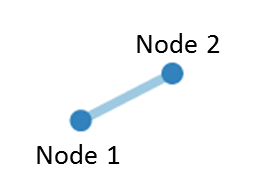
\includegraphics{images/samplegraph.png}
\caption{\label{fig:samplegraph} Graph created from sample gml file.}
\end{figure}
The second use of igraph within gravicom is to compute initial $x$ and $y$ coordinates for the nodes of the graph using a force-driven layout. This provides the initialization for the force-layout algorithm in D3. This reduces the computational load on the clients' side and helps minimize unnecessary movement by the nodes. This is critical as the extra movement at the loading of the pages creates an unnecessarily chaotic start to the user's experience. 




\section{Further Work}

In this section, we will briefly cover two ideas for extending our work on gravicom.  The first, integrated algorithmic community detection, improves community detection, and the second, dynamic temporal graph visualization, will allow for the analysis of changing graphs over time in gravicom.

\subsection{Integrated Algorithmic Community Detection}
The idea behind integrated algorithmic community detection is to combine the benefits of human detection of communities with algorithmic detection. Human detection using gravicom as described in this paper can serve as an initialization phase of community detection. From there, an iterative algoritm would be available to run in the background. The algorithm would run step-by-step and send results back to the user for two purposes. First, the user can visually track how the algorithm is detecting communities by showing what groups are created when. That transition helps the user track progression with the algorithm.  Being able to visually track changes will help the user understand what is going on with the algorithm, rather than a black box method. 

Second, in between iterations of the algorithm, the user can choose to accept or reject changes made by the algorithm. The user could make adjustments and send the updated results back to the algorithm. This checkpoint would in effect create flexible stopping criteria.  For example, suppose the algorithm, running step-by-step, still has remaining steps before meeting the stopping criteria.  A user could decide at each point whether to continue through the remaining steps or stop at a specific point.  Similarly, suppose the algorithm has met the stopping criteria but the user identifies the need to perform additional iterations.  The integration of human and algorithmic detection would allow the user to stop or continue as necessary.

Because we built gravicom on the shiny framework, it is not a major step to add this feature. We already have the ability to send a current graph's status to R running on the server, perform manipulations, and send the graph back. The next step would be to implement the algorithm in R, using, for example, the igraph package.

\subsection{Dynamic Temporal Graph Visualization}
The idea for dynamic temporal graph visualization is that a user would be able to view a dynamic graph across time, specifically how the edges change between nodes. With this, a user could find time-dependent communities. 

An example that illustrates this point is the series of novels, A Song of Ice and Fire \cite{martin1996game, martin1998clash, martin2000storm, martin2005feast, martin2011dance}. This data was compiled by Jerome Cukier using two fan-maintained ressources on the series \cite{cukier2012got}. Looking at important events in the same chapter, one could look at how relationships between characters are changing from one chapter to the next. We performed this analysis for each book separately and we present the results in Figure~\ref{fig:further_got}. The first thing that stands out from this visualization is a stark difference in how characters interact from book two to book three. Book two there are many medium sized clusters in evidence, meaning many disparate events affecting a mid size amoutn of characters. To the contrary, book 3 shows one very large event occuring and then many other events affecting a small amount of characters. In fact, the third book in the series, A Storm of Swords, houses a brutal massacre in which over 10 major characters are killed. 

\begin{figure}[H]
\centering
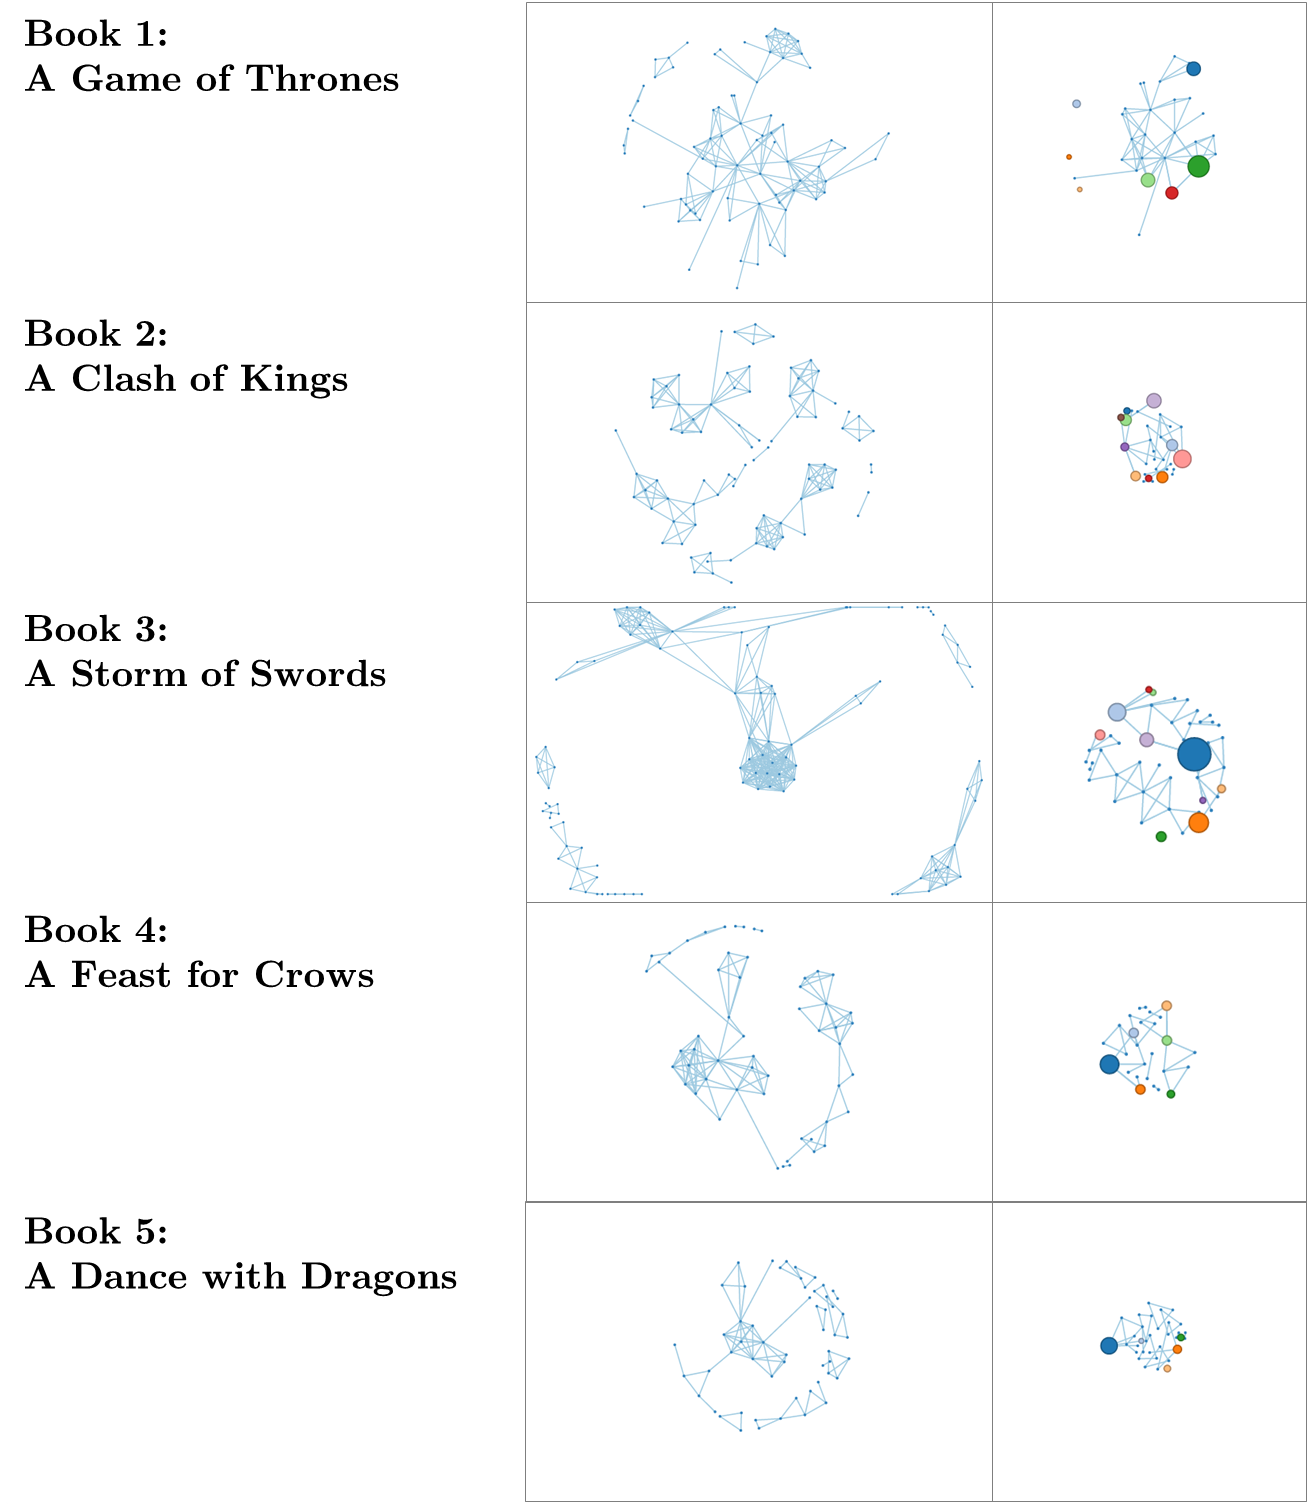
\includegraphics[width=\textwidth]{images/further_got.png}
\caption{\label{fig:further_got} A look at the relationships between characters over time for all five books in A Song of Ice and Fire by George R. R. Martin in terms of mutual events.}
\end{figure}

The piece that is missing with the analysis is the ability to track the change of character's relationships from one book to the next. 


\printbibliography
\end{document}
